\documentclass{extbook}[14pt]
\usepackage{multicol, enumerate, enumitem, hyperref, color, soul, setspace, parskip, fancyhdr, amssymb, amsthm, amsmath, latexsym, units, mathtools}
\everymath{\displaystyle}
\usepackage[headsep=0.5cm,headheight=0cm, left=1 in,right= 1 in,top= 1 in,bottom= 1 in]{geometry}
\usepackage{dashrule}  % Package to use the command below to create lines between items
\newcommand{\litem}[1]{\item #1

\rule{\textwidth}{0.4pt}}
\pagestyle{fancy}
\lhead{}
\chead{Answer Key for Makeup Progress Quiz 2 Version ALL}
\rhead{}
\lfoot{2790-1423}
\cfoot{}
\rfoot{Summer C 2021}
\begin{document}
\textbf{This key should allow you to understand why you choose the option you did (beyond just getting a question right or wrong). \href{https://xronos.clas.ufl.edu/mac1105spring2020/courseDescriptionAndMisc/Exams/LearningFromResults}{More instructions on how to use this key can be found here}.}

\textbf{If you have a suggestion to make the keys better, \href{https://forms.gle/CZkbZmPbC9XALEE88}{please fill out the short survey here}.}

\textit{Note: This key is auto-generated and may contain issues and/or errors. The keys are reviewed after each exam to ensure grading is done accurately. If there are issues (like duplicate options), they are noted in the offline gradebook. The keys are a work-in-progress to give students as many resources to improve as possible.}

\rule{\textwidth}{0.4pt}

\begin{enumerate}\litem{
Which of the following equations \textit{could} be of the graph presented below?

\begin{center}
    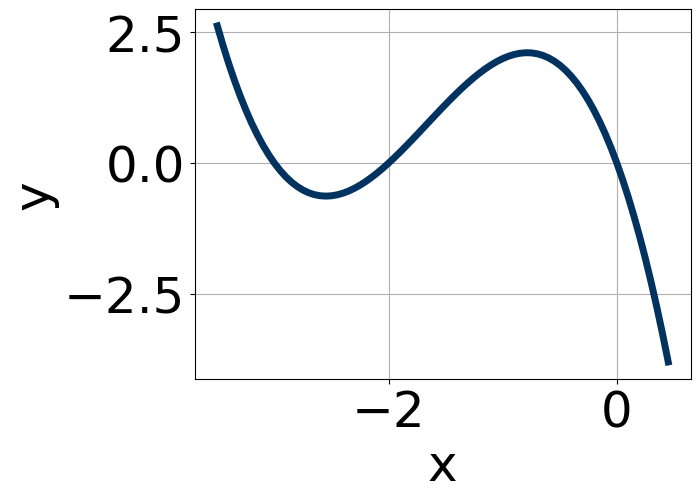
\includegraphics[width=0.5\textwidth]{../Figures/polyGraphToFunctionA.png}
\end{center}


The solution is \( -19x^{11} (x + 2)^{9} (x + 3)^{9} \), which is option A.\begin{enumerate}[label=\Alph*.]
\item \( -19x^{11} (x + 2)^{9} (x + 3)^{9} \)

* This is the correct option.
\item \( 8x^{7} (x + 2)^{11} (x + 3)^{9} \)

This corresponds to the leading coefficient being the opposite value than it should be.
\item \( -2x^{9} (x + 2)^{10} (x + 3)^{8} \)

The factors $-2$ and $-3$ have have been odd power.
\item \( -19x^{5} (x + 2)^{8} (x + 3)^{9} \)

The factor $-2$ should have been an odd power.
\item \( 15x^{9} (x + 2)^{6} (x + 3)^{7} \)

The factor $(x + 2)$ should have an odd power and the leading coefficient should be the opposite sign.
\end{enumerate}

\textbf{General Comment:} General Comments: Draw the x-axis to determine which zeros are touching (and so have even multiplicity) or cross (and have odd multiplicity).
}
\litem{
Construct the lowest-degree polynomial given the zeros below. Then, choose the intervals that contain the coefficients of the polynomial in the form $ax^3+bx^2+cx+d$.
\[ \frac{-3}{2}, -7, \text{ and } \frac{7}{2} \]The solution is \( 4x^{3} +20 x^{2} -77 x -147 \), which is option A.\begin{enumerate}[label=\Alph*.]
\item \( a \in [1, 7], b \in [20, 23], c \in [-77, -71], \text{ and } d \in [-149, -143] \)

* $4x^{3} +20 x^{2} -77 x -147$, which is the correct option.
\item \( a \in [1, 7], b \in [-20, -13], c \in [-77, -71], \text{ and } d \in [147, 150] \)

$4x^{3} -20 x^{2} -77 x + 147$, which corresponds to multiplying out $(2x -3)(x -7)(2x + 7)$.
\item \( a \in [1, 7], b \in [6, 15], c \in [-120, -118], \text{ and } d \in [147, 150] \)

$4x^{3} +8 x^{2} -119 x + 147$, which corresponds to multiplying out $(2x -3)(x + 7)(2x -7)$.
\item \( a \in [1, 7], b \in [20, 23], c \in [-77, -71], \text{ and } d \in [147, 150] \)

$4x^{3} +20 x^{2} -77 x + 147$, which corresponds to multiplying everything correctly except the constant term.
\item \( a \in [1, 7], b \in [-52, -47], c \in [158, 164], \text{ and } d \in [-149, -143] \)

$4x^{3} -48 x^{2} +161 x -147$, which corresponds to multiplying out $(2x -3)(x -7)(2x -7)$.
\end{enumerate}

\textbf{General Comment:} To construct the lowest-degree polynomial, you want to multiply out $(2x + 3)(x + 7)(2x -7)$
}
\litem{
Describe the zero behavior of the zero $x = -7$ of the polynomial below.
\[ f(x) = -2(x - 4)^{8}(x + 4)^{5}(x + 7)^{10}(x - 7)^{9} \]The solution is the graph below, which is option B.
    \begin{center}
        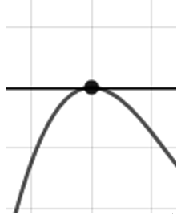
\includegraphics[width=0.3\textwidth]{../Figures/polyZeroBehaviorCopyBA.png}
    \end{center}\begin{enumerate}[label=\Alph*.]
\begin{multicols}{2}
\item 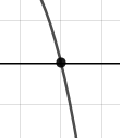
\includegraphics[width = 0.3\textwidth]{../Figures/polyZeroBehaviorCopyAA.png}
\item 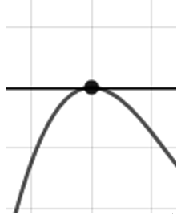
\includegraphics[width = 0.3\textwidth]{../Figures/polyZeroBehaviorCopyBA.png}
\item 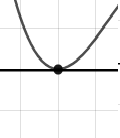
\includegraphics[width = 0.3\textwidth]{../Figures/polyZeroBehaviorCopyCA.png}
\item 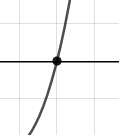
\includegraphics[width = 0.3\textwidth]{../Figures/polyZeroBehaviorCopyDA.png}
\end{multicols}\item None of the above.\end{enumerate}
\textbf{General Comment:} You will need to sketch the entire graph, then zoom in on the zero the question asks about.
}
\litem{
Describe the end behavior of the polynomial below.
\[ f(x) = 7(x - 7)^{2}(x + 7)^{3}(x - 8)^{5}(x + 8)^{5} \]The solution is the graph below, which is option D.
    \begin{center}
        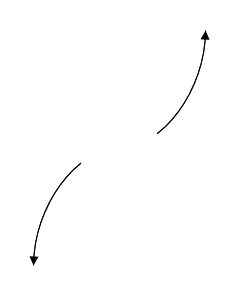
\includegraphics[width=0.3\textwidth]{../Figures/polyEndBehaviorCopyDA.png}
    \end{center}\begin{enumerate}[label=\Alph*.]
\begin{multicols}{2}
\item 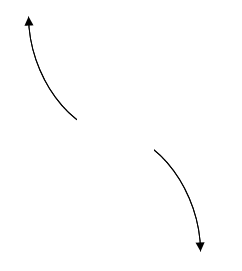
\includegraphics[width = 0.3\textwidth]{../Figures/polyEndBehaviorCopyAA.png}
\item 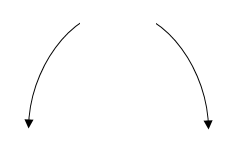
\includegraphics[width = 0.3\textwidth]{../Figures/polyEndBehaviorCopyBA.png}
\item 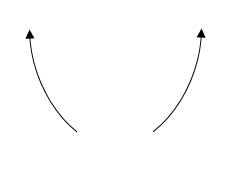
\includegraphics[width = 0.3\textwidth]{../Figures/polyEndBehaviorCopyCA.png}
\item 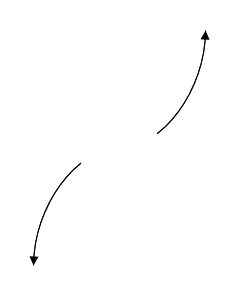
\includegraphics[width = 0.3\textwidth]{../Figures/polyEndBehaviorCopyDA.png}
\end{multicols}\item None of the above.\end{enumerate}
\textbf{General Comment:} Remember that end behavior is determined by the leading coefficient AND whether the \textbf{sum} of the multiplicities is positive or negative.
}
\litem{
Describe the end behavior of the polynomial below.
\[ f(x) = 2(x - 2)^{4}(x + 2)^{7}(x - 4)^{2}(x + 4)^{2} \]The solution is the graph below, which is option D.
    \begin{center}
        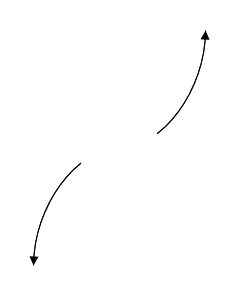
\includegraphics[width=0.3\textwidth]{../Figures/polyEndBehaviorDA.png}
    \end{center}\begin{enumerate}[label=\Alph*.]
\begin{multicols}{2}
\item 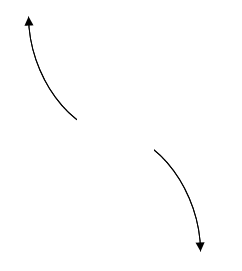
\includegraphics[width = 0.3\textwidth]{../Figures/polyEndBehaviorAA.png}
\item 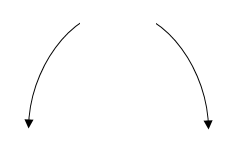
\includegraphics[width = 0.3\textwidth]{../Figures/polyEndBehaviorBA.png}
\item 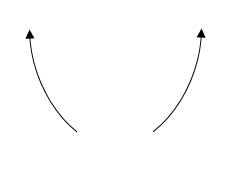
\includegraphics[width = 0.3\textwidth]{../Figures/polyEndBehaviorCA.png}
\item 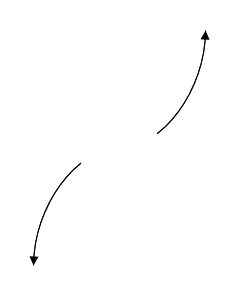
\includegraphics[width = 0.3\textwidth]{../Figures/polyEndBehaviorDA.png}
\end{multicols}\item None of the above.\end{enumerate}
\textbf{General Comment:} Remember that end behavior is determined by the leading coefficient AND whether the \textbf{sum} of the multiplicities is positive or negative.
}
\litem{
Construct the lowest-degree polynomial given the zeros below. Then, choose the intervals that contain the coefficients of the polynomial in the form $x^3+bx^2+cx+d$.
\[ -4 + 4 i \text{ and } 4 \]The solution is \( x^{3} +4 x^{2} -128 \), which is option D.\begin{enumerate}[label=\Alph*.]
\item \( b \in [0.9, 3.2], c \in [-3, 3], \text{ and } d \in [-18, -14] \)

$x^{3} + x^{2} -16$, which corresponds to multiplying out $(x + 4)(x -4)$.
\item \( b \in [0.9, 3.2], c \in [-10, -7], \text{ and } d \in [13, 21] \)

$x^{3} + x^{2} -8 x + 16$, which corresponds to multiplying out $(x -4)(x -4)$.
\item \( b \in [-7.8, -3.9], c \in [-3, 3], \text{ and } d \in [121, 134] \)

$x^{3} -4 x^{2} + 128$, which corresponds to multiplying out $(x-(-4 + 4 i))(x-(-4 - 4 i))(x + 4)$.
\item \( b \in [3.1, 5.5], c \in [-3, 3], \text{ and } d \in [-130, -123] \)

* $x^{3} +4 x^{2} -128$, which is the correct option.
\item \( \text{None of the above.} \)

This corresponds to making an unanticipated error or not understanding how to use nonreal complex numbers to create the lowest-degree polynomial. If you chose this and are not sure what you did wrong, please contact the coordinator for help.
\end{enumerate}

\textbf{General Comment:} Remember that the conjugate of $a+bi$ is $a-bi$. Since these zeros always come in pairs, we need to multiply out $(x-(-4 + 4 i))(x-(-4 - 4 i))(x-(4))$.
}
\litem{
Construct the lowest-degree polynomial given the zeros below. Then, choose the intervals that contain the coefficients of the polynomial in the form $ax^3+bx^2+cx+d$.
\[ -3, \frac{-5}{2}, \text{ and } \frac{-1}{5} \]The solution is \( 10x^{3} +57 x^{2} +86 x + 15 \), which is option A.\begin{enumerate}[label=\Alph*.]
\item \( a \in [10, 15], b \in [51, 61], c \in [80, 87], \text{ and } d \in [11, 19] \)

* $10x^{3} +57 x^{2} +86 x + 15$, which is the correct option.
\item \( a \in [10, 15], b \in [-53, -46], c \in [53, 71], \text{ and } d \in [11, 19] \)

$10x^{3} -53 x^{2} +64 x + 15$, which corresponds to multiplying out $(x -3)(2x -5)(5x + 1)$.
\item \( a \in [10, 15], b \in [-57, -54], c \in [80, 87], \text{ and } d \in [-17, -7] \)

$10x^{3} -57 x^{2} +86 x -15$, which corresponds to multiplying out $(x -3)(2x -5)(5x -1)$.
\item \( a \in [10, 15], b \in [-3, 6], c \in [-81, -75], \text{ and } d \in [-17, -7] \)

$10x^{3} -3 x^{2} -76 x -15$, which corresponds to multiplying out $(x -3)(2x + 5)(5x + 1)$.
\item \( a \in [10, 15], b \in [51, 61], c \in [80, 87], \text{ and } d \in [-17, -7] \)

$10x^{3} +57 x^{2} +86 x -15$, which corresponds to multiplying everything correctly except the constant term.
\end{enumerate}

\textbf{General Comment:} To construct the lowest-degree polynomial, you want to multiply out $(x + 3)(2x + 5)(5x + 1)$
}
\litem{
Which of the following equations \textit{could} be of the graph presented below?

\begin{center}
    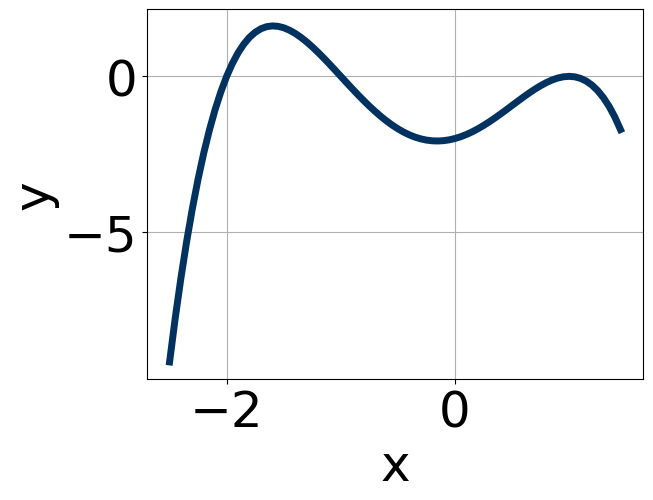
\includegraphics[width=0.5\textwidth]{../Figures/polyGraphToFunctionCopyA.png}
\end{center}


The solution is \( -15(x - 1)^{8} (x + 1)^{11} (x + 2)^{7} \), which is option A.\begin{enumerate}[label=\Alph*.]
\item \( -15(x - 1)^{8} (x + 1)^{11} (x + 2)^{7} \)

* This is the correct option.
\item \( -11(x - 1)^{8} (x + 1)^{6} (x + 2)^{9} \)

The factor $(x + 1)$ should have an odd power.
\item \( 16(x - 1)^{8} (x + 1)^{9} (x + 2)^{11} \)

This corresponds to the leading coefficient being the opposite value than it should be.
\item \( -14(x - 1)^{7} (x + 1)^{8} (x + 2)^{9} \)

The factor $1$ should have an even power and the factor $-1$ should have an odd power.
\item \( 11(x - 1)^{4} (x + 1)^{11} (x + 2)^{4} \)

The factor $(x + 2)$ should have an odd power and the leading coefficient should be the opposite sign.
\end{enumerate}

\textbf{General Comment:} General Comments: Draw the x-axis to determine which zeros are touching (and so have even multiplicity) or cross (and have odd multiplicity).
}
\litem{
Construct the lowest-degree polynomial given the zeros below. Then, choose the intervals that contain the coefficients of the polynomial in the form $x^3+bx^2+cx+d$.
\[ -3 - 4 i \text{ and } -2 \]The solution is \( x^{3} +8 x^{2} +37 x + 50 \), which is option C.\begin{enumerate}[label=\Alph*.]
\item \( b \in [-1, 5], c \in [1.8, 5.3], \text{ and } d \in [5.8, 6.4] \)

$x^{3} + x^{2} +5 x + 6$, which corresponds to multiplying out $(x + 3)(x + 2)$.
\item \( b \in [-1, 5], c \in [5.2, 8.8], \text{ and } d \in [7.7, 10.7] \)

$x^{3} + x^{2} +6 x + 8$, which corresponds to multiplying out $(x + 4)(x + 2)$.
\item \( b \in [4, 9], c \in [35.8, 38.9], \text{ and } d \in [46.8, 52.1] \)

* $x^{3} +8 x^{2} +37 x + 50$, which is the correct option.
\item \( b \in [-9, -3], c \in [35.8, 38.9], \text{ and } d \in [-50.4, -49] \)

$x^{3} -8 x^{2} +37 x -50$, which corresponds to multiplying out $(x-(-3 - 4 i))(x-(-3 + 4 i))(x -2)$.
\item \( \text{None of the above.} \)

This corresponds to making an unanticipated error or not understanding how to use nonreal complex numbers to create the lowest-degree polynomial. If you chose this and are not sure what you did wrong, please contact the coordinator for help.
\end{enumerate}

\textbf{General Comment:} Remember that the conjugate of $a+bi$ is $a-bi$. Since these zeros always come in pairs, we need to multiply out $(x-(-3 - 4 i))(x-(-3 + 4 i))(x-(-2))$.
}
\litem{
Describe the zero behavior of the zero $x = -8$ of the polynomial below.
\[ f(x) = -2(x - 8)^{8}(x + 8)^{11}(x + 9)^{9}(x - 9)^{13} \]The solution is the graph below, which is option D.
    \begin{center}
        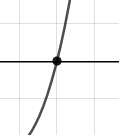
\includegraphics[width=0.3\textwidth]{../Figures/polyZeroBehaviorDA.png}
    \end{center}\begin{enumerate}[label=\Alph*.]
\begin{multicols}{2}
\item 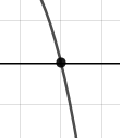
\includegraphics[width = 0.3\textwidth]{../Figures/polyZeroBehaviorAA.png}
\item 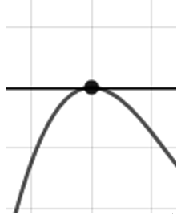
\includegraphics[width = 0.3\textwidth]{../Figures/polyZeroBehaviorBA.png}
\item 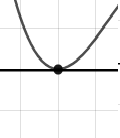
\includegraphics[width = 0.3\textwidth]{../Figures/polyZeroBehaviorCA.png}
\item 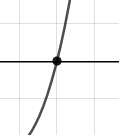
\includegraphics[width = 0.3\textwidth]{../Figures/polyZeroBehaviorDA.png}
\end{multicols}\item None of the above.\end{enumerate}
\textbf{General Comment:} You will need to sketch the entire graph, then zoom in on the zero the question asks about.
}
\litem{
Which of the following equations \textit{could} be of the graph presented below?

\begin{center}
    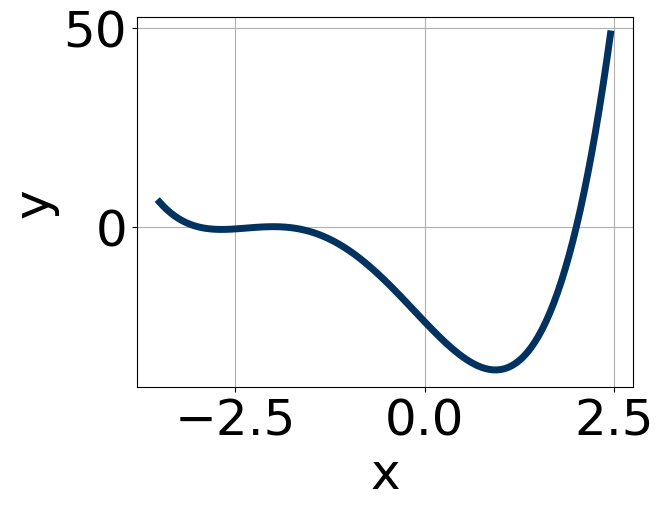
\includegraphics[width=0.5\textwidth]{../Figures/polyGraphToFunctionB.png}
\end{center}


The solution is \( 13(x + 2)^{4} (x - 2)^{11} (x + 3)^{11} \), which is option C.\begin{enumerate}[label=\Alph*.]
\item \( 19(x + 2)^{7} (x - 2)^{4} (x + 3)^{9} \)

The factor $-2$ should have an even power and the factor $2$ should have an odd power.
\item \( 20(x + 2)^{10} (x - 2)^{8} (x + 3)^{7} \)

The factor $(x - 2)$ should have an odd power.
\item \( 13(x + 2)^{4} (x - 2)^{11} (x + 3)^{11} \)

* This is the correct option.
\item \( -18(x + 2)^{4} (x - 2)^{7} (x + 3)^{4} \)

The factor $(x + 3)$ should have an odd power and the leading coefficient should be the opposite sign.
\item \( -4(x + 2)^{10} (x - 2)^{11} (x + 3)^{5} \)

This corresponds to the leading coefficient being the opposite value than it should be.
\end{enumerate}

\textbf{General Comment:} General Comments: Draw the x-axis to determine which zeros are touching (and so have even multiplicity) or cross (and have odd multiplicity).
}
\litem{
Construct the lowest-degree polynomial given the zeros below. Then, choose the intervals that contain the coefficients of the polynomial in the form $ax^3+bx^2+cx+d$.
\[ \frac{1}{4}, \frac{7}{5}, \text{ and } 2 \]The solution is \( 20x^{3} -73 x^{2} +73 x -14 \), which is option C.\begin{enumerate}[label=\Alph*.]
\item \( a \in [17, 26], b \in [68, 75], c \in [69, 74], \text{ and } d \in [10, 16] \)

$20x^{3} +73 x^{2} +73 x + 14$, which corresponds to multiplying out $(4x + 1)(5x + 7)(x + 2)$.
\item \( a \in [17, 26], b \in [-7, -6], c \in [-59, -56], \text{ and } d \in [-18, -13] \)

$20x^{3} -7 x^{2} -59 x -14$, which corresponds to multiplying out $(4x + 1)(5x + 7)(x -2)$.
\item \( a \in [17, 26], b \in [-73, -66], c \in [69, 74], \text{ and } d \in [-18, -13] \)

* $20x^{3} -73 x^{2} +73 x -14$, which is the correct option.
\item \( a \in [17, 26], b \in [-73, -66], c \in [69, 74], \text{ and } d \in [10, 16] \)

$20x^{3} -73 x^{2} +73 x + 14$, which corresponds to multiplying everything correctly except the constant term.
\item \( a \in [17, 26], b \in [-66, -58], c \in [34, 45], \text{ and } d \in [10, 16] \)

$20x^{3} -63 x^{2} +39 x + 14$, which corresponds to multiplying out $(4x + 1)(5x -7)(x -2)$.
\end{enumerate}

\textbf{General Comment:} To construct the lowest-degree polynomial, you want to multiply out $(4x -1)(5x -7)(x -2)$
}
\litem{
Describe the zero behavior of the zero $x = 2$ of the polynomial below.
\[ f(x) = -9(x - 7)^{7}(x + 7)^{4}(x - 2)^{12}(x + 2)^{9} \]The solution is the graph below, which is option C.
    \begin{center}
        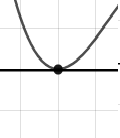
\includegraphics[width=0.3\textwidth]{../Figures/polyZeroBehaviorCopyCB.png}
    \end{center}\begin{enumerate}[label=\Alph*.]
\begin{multicols}{2}
\item 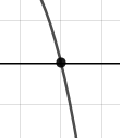
\includegraphics[width = 0.3\textwidth]{../Figures/polyZeroBehaviorCopyAB.png}
\item 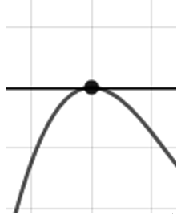
\includegraphics[width = 0.3\textwidth]{../Figures/polyZeroBehaviorCopyBB.png}
\item 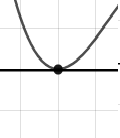
\includegraphics[width = 0.3\textwidth]{../Figures/polyZeroBehaviorCopyCB.png}
\item 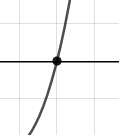
\includegraphics[width = 0.3\textwidth]{../Figures/polyZeroBehaviorCopyDB.png}
\end{multicols}\item None of the above.\end{enumerate}
\textbf{General Comment:} You will need to sketch the entire graph, then zoom in on the zero the question asks about.
}
\litem{
Describe the end behavior of the polynomial below.
\[ f(x) = 8(x - 9)^{2}(x + 9)^{5}(x - 7)^{4}(x + 7)^{6} \]The solution is the graph below, which is option D.
    \begin{center}
        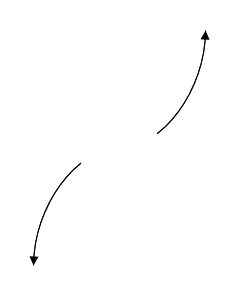
\includegraphics[width=0.3\textwidth]{../Figures/polyEndBehaviorCopyDB.png}
    \end{center}\begin{enumerate}[label=\Alph*.]
\begin{multicols}{2}
\item 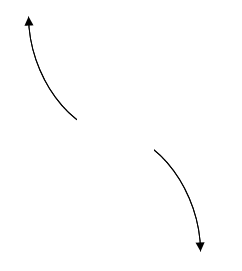
\includegraphics[width = 0.3\textwidth]{../Figures/polyEndBehaviorCopyAB.png}
\item 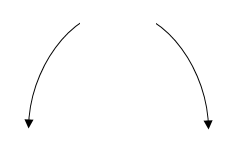
\includegraphics[width = 0.3\textwidth]{../Figures/polyEndBehaviorCopyBB.png}
\item 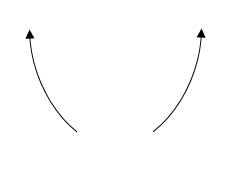
\includegraphics[width = 0.3\textwidth]{../Figures/polyEndBehaviorCopyCB.png}
\item 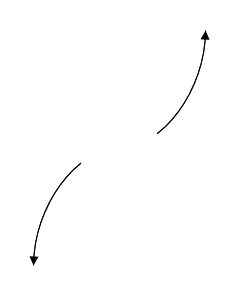
\includegraphics[width = 0.3\textwidth]{../Figures/polyEndBehaviorCopyDB.png}
\end{multicols}\item None of the above.\end{enumerate}
\textbf{General Comment:} Remember that end behavior is determined by the leading coefficient AND whether the \textbf{sum} of the multiplicities is positive or negative.
}
\litem{
Describe the end behavior of the polynomial below.
\[ f(x) = 9(x + 5)^{3}(x - 5)^{6}(x - 3)^{5}(x + 3)^{7} \]The solution is the graph below, which is option D.
    \begin{center}
        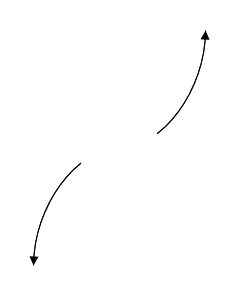
\includegraphics[width=0.3\textwidth]{../Figures/polyEndBehaviorDB.png}
    \end{center}\begin{enumerate}[label=\Alph*.]
\begin{multicols}{2}
\item 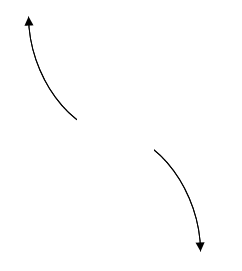
\includegraphics[width = 0.3\textwidth]{../Figures/polyEndBehaviorAB.png}
\item 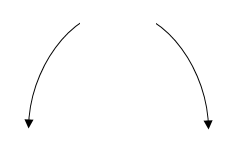
\includegraphics[width = 0.3\textwidth]{../Figures/polyEndBehaviorBB.png}
\item 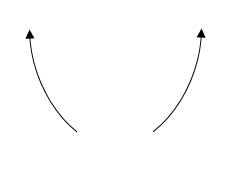
\includegraphics[width = 0.3\textwidth]{../Figures/polyEndBehaviorCB.png}
\item 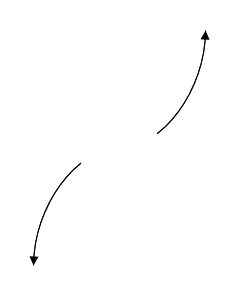
\includegraphics[width = 0.3\textwidth]{../Figures/polyEndBehaviorDB.png}
\end{multicols}\item None of the above.\end{enumerate}
\textbf{General Comment:} Remember that end behavior is determined by the leading coefficient AND whether the \textbf{sum} of the multiplicities is positive or negative.
}
\litem{
Construct the lowest-degree polynomial given the zeros below. Then, choose the intervals that contain the coefficients of the polynomial in the form $x^3+bx^2+cx+d$.
\[ -2 + 5 i \text{ and } 3 \]The solution is \( x^{3} + x^{2} +17 x -87 \), which is option A.\begin{enumerate}[label=\Alph*.]
\item \( b \in [-0.1, 2.4], c \in [15, 24], \text{ and } d \in [-94, -80] \)

* $x^{3} + x^{2} +17 x -87$, which is the correct option.
\item \( b \in [-2.5, -0.9], c \in [15, 24], \text{ and } d \in [75, 89] \)

$x^{3} -1 x^{2} +17 x + 87$, which corresponds to multiplying out $(x-(-2 + 5 i))(x-(-2 - 5 i))(x + 3)$.
\item \( b \in [-0.1, 2.4], c \in [-8, -3], \text{ and } d \in [10, 24] \)

$x^{3} + x^{2} -8 x + 15$, which corresponds to multiplying out $(x -5)(x -3)$.
\item \( b \in [-0.1, 2.4], c \in [-2, 5], \text{ and } d \in [-10, -2] \)

$x^{3} + x^{2} -x -6$, which corresponds to multiplying out $(x + 2)(x -3)$.
\item \( \text{None of the above.} \)

This corresponds to making an unanticipated error or not understanding how to use nonreal complex numbers to create the lowest-degree polynomial. If you chose this and are not sure what you did wrong, please contact the coordinator for help.
\end{enumerate}

\textbf{General Comment:} Remember that the conjugate of $a+bi$ is $a-bi$. Since these zeros always come in pairs, we need to multiply out $(x-(-2 + 5 i))(x-(-2 - 5 i))(x-(3))$.
}
\litem{
Construct the lowest-degree polynomial given the zeros below. Then, choose the intervals that contain the coefficients of the polynomial in the form $ax^3+bx^2+cx+d$.
\[ \frac{-3}{2}, \frac{-7}{3}, \text{ and } -4 \]The solution is \( 6x^{3} +47 x^{2} +113 x + 84 \), which is option D.\begin{enumerate}[label=\Alph*.]
\item \( a \in [1, 13], b \in [42, 51], c \in [111, 117], \text{ and } d \in [-87, -83] \)

$6x^{3} +47 x^{2} +113 x -84$, which corresponds to multiplying everything correctly except the constant term.
\item \( a \in [1, 13], b \in [-4, 2], c \in [-76, -68], \text{ and } d \in [84, 88] \)

$6x^{3} + x^{2} -71 x + 84$, which corresponds to multiplying out $(2x -3)(3x -7)(x + 4)$.
\item \( a \in [1, 13], b \in [-50, -41], c \in [111, 117], \text{ and } d \in [-87, -83] \)

$6x^{3} -47 x^{2} +113 x -84$, which corresponds to multiplying out $(2x -3)(3x -7)(x -4)$.
\item \( a \in [1, 13], b \in [42, 51], c \in [111, 117], \text{ and } d \in [84, 88] \)

* $6x^{3} +47 x^{2} +113 x + 84$, which is the correct option.
\item \( a \in [1, 13], b \in [28, 30], c \in [-3, 5], \text{ and } d \in [-87, -83] \)

$6x^{3} +29 x^{2} -x -84$, which corresponds to multiplying out $(2x -3)(3x + 7)(x + 4)$.
\end{enumerate}

\textbf{General Comment:} To construct the lowest-degree polynomial, you want to multiply out $(2x + 3)(3x + 7)(x + 4)$
}
\litem{
Which of the following equations \textit{could} be of the graph presented below?

\begin{center}
    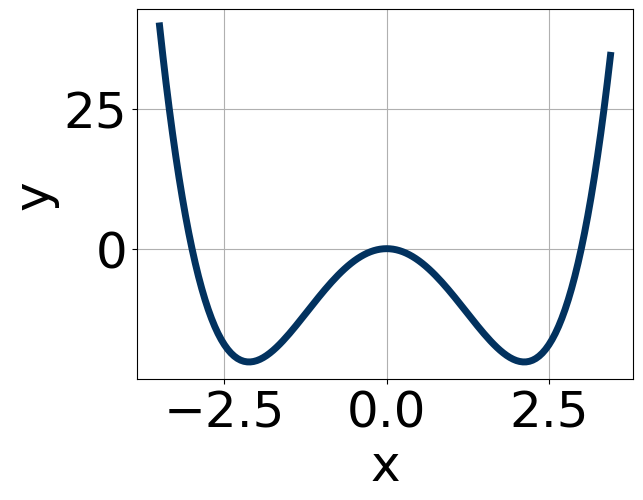
\includegraphics[width=0.5\textwidth]{../Figures/polyGraphToFunctionCopyB.png}
\end{center}


The solution is \( 18x^{8} (x + 3)^{9} (x - 3)^{7} \), which is option A.\begin{enumerate}[label=\Alph*.]
\item \( 18x^{8} (x + 3)^{9} (x - 3)^{7} \)

* This is the correct option.
\item \( -19x^{4} (x + 3)^{5} (x - 3)^{4} \)

The factor $(x - 3)$ should have an odd power and the leading coefficient should be the opposite sign.
\item \( 19x^{4} (x + 3)^{8} (x - 3)^{11} \)

The factor $(x + 3)$ should have an odd power.
\item \( 8x^{5} (x + 3)^{8} (x - 3)^{7} \)

The factor $0$ should have an even power and the factor $-3$ should have an odd power.
\item \( -3x^{4} (x + 3)^{11} (x - 3)^{7} \)

This corresponds to the leading coefficient being the opposite value than it should be.
\end{enumerate}

\textbf{General Comment:} General Comments: Draw the x-axis to determine which zeros are touching (and so have even multiplicity) or cross (and have odd multiplicity).
}
\litem{
Construct the lowest-degree polynomial given the zeros below. Then, choose the intervals that contain the coefficients of the polynomial in the form $x^3+bx^2+cx+d$.
\[ 5 + 2 i \text{ and } 4 \]The solution is \( x^{3} -14 x^{2} +69 x -116 \), which is option B.\begin{enumerate}[label=\Alph*.]
\item \( b \in [-6, 2], c \in [-9.4, -7.5], \text{ and } d \in [18, 22] \)

$x^{3} + x^{2} -9 x + 20$, which corresponds to multiplying out $(x -5)(x -4)$.
\item \( b \in [-21, -8], c \in [67.5, 70.9], \text{ and } d \in [-126, -113] \)

* $x^{3} -14 x^{2} +69 x -116$, which is the correct option.
\item \( b \in [-6, 2], c \in [-8, -3.8], \text{ and } d \in [5, 12] \)

$x^{3} + x^{2} -6 x + 8$, which corresponds to multiplying out $(x -2)(x -4)$.
\item \( b \in [12, 21], c \in [67.5, 70.9], \text{ and } d \in [115, 119] \)

$x^{3} +14 x^{2} +69 x + 116$, which corresponds to multiplying out $(x-(5 + 2 i))(x-(5 - 2 i))(x + 4)$.
\item \( \text{None of the above.} \)

This corresponds to making an unanticipated error or not understanding how to use nonreal complex numbers to create the lowest-degree polynomial. If you chose this and are not sure what you did wrong, please contact the coordinator for help.
\end{enumerate}

\textbf{General Comment:} Remember that the conjugate of $a+bi$ is $a-bi$. Since these zeros always come in pairs, we need to multiply out $(x-(5 + 2 i))(x-(5 - 2 i))(x-(4))$.
}
\litem{
Describe the zero behavior of the zero $x = 2$ of the polynomial below.
\[ f(x) = 8(x + 2)^{2}(x - 2)^{7}(x - 4)^{9}(x + 4)^{11} \]The solution is the graph below, which is option A.
    \begin{center}
        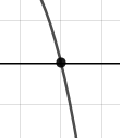
\includegraphics[width=0.3\textwidth]{../Figures/polyZeroBehaviorAB.png}
    \end{center}\begin{enumerate}[label=\Alph*.]
\begin{multicols}{2}
\item 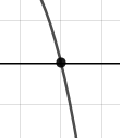
\includegraphics[width = 0.3\textwidth]{../Figures/polyZeroBehaviorAB.png}
\item 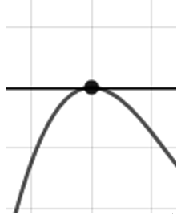
\includegraphics[width = 0.3\textwidth]{../Figures/polyZeroBehaviorBB.png}
\item 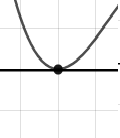
\includegraphics[width = 0.3\textwidth]{../Figures/polyZeroBehaviorCB.png}
\item 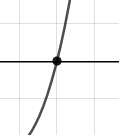
\includegraphics[width = 0.3\textwidth]{../Figures/polyZeroBehaviorDB.png}
\end{multicols}\item None of the above.\end{enumerate}
\textbf{General Comment:} You will need to sketch the entire graph, then zoom in on the zero the question asks about.
}
\litem{
Which of the following equations \textit{could} be of the graph presented below?

\begin{center}
    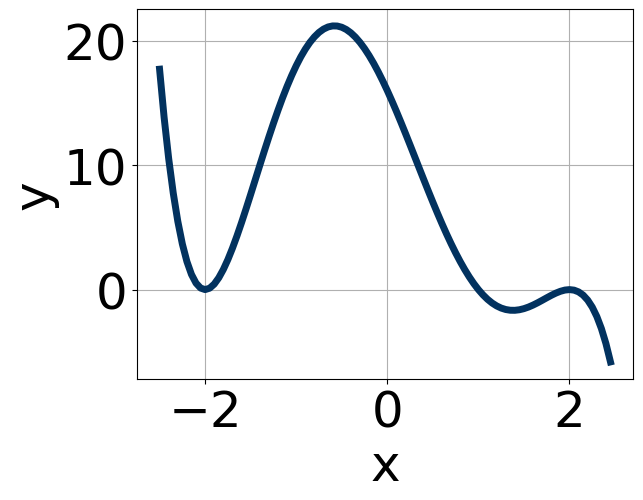
\includegraphics[width=0.5\textwidth]{../Figures/polyGraphToFunctionC.png}
\end{center}


The solution is \( -6(x - 2)^{10} (x + 2)^{4} (x - 1)^{7} \), which is option D.\begin{enumerate}[label=\Alph*.]
\item \( -13(x - 2)^{10} (x + 2)^{5} (x - 1)^{10} \)

The factor $(x + 2)$ should have an even power and the factor $(x - 1)$ should have an odd power.
\item \( -14(x - 2)^{10} (x + 2)^{9} (x - 1)^{11} \)

The factor $(x + 2)$ should have an even power.
\item \( 18(x - 2)^{10} (x + 2)^{4} (x - 1)^{10} \)

The factor $(x - 1)$ should have an odd power and the leading coefficient should be the opposite sign.
\item \( -6(x - 2)^{10} (x + 2)^{4} (x - 1)^{7} \)

* This is the correct option.
\item \( 16(x - 2)^{8} (x + 2)^{8} (x - 1)^{5} \)

This corresponds to the leading coefficient being the opposite value than it should be.
\end{enumerate}

\textbf{General Comment:} General Comments: Draw the x-axis to determine which zeros are touching (and so have even multiplicity) or cross (and have odd multiplicity).
}
\litem{
Construct the lowest-degree polynomial given the zeros below. Then, choose the intervals that contain the coefficients of the polynomial in the form $ax^3+bx^2+cx+d$.
\[ \frac{-3}{5}, \frac{7}{4}, \text{ and } \frac{1}{3} \]The solution is \( 60x^{3} -89 x^{2} -40 x + 21 \), which is option B.\begin{enumerate}[label=\Alph*.]
\item \( a \in [53, 63], b \in [-91, -78], c \in [-46, -37], \text{ and } d \in [-21, -18] \)

$60x^{3} -89 x^{2} -40 x -21$, which corresponds to multiplying everything correctly except the constant term.
\item \( a \in [53, 63], b \in [-91, -78], c \in [-46, -37], \text{ and } d \in [20, 23] \)

* $60x^{3} -89 x^{2} -40 x + 21$, which is the correct option.
\item \( a \in [53, 63], b \in [83, 95], c \in [-46, -37], \text{ and } d \in [-21, -18] \)

$60x^{3} +89 x^{2} -40 x -21$, which corresponds to multiplying out $(5x -3)(4x + 7)(3x + 1)$.
\item \( a \in [53, 63], b \in [49, 51], c \in [-88, -79], \text{ and } d \in [20, 23] \)

$60x^{3} +49 x^{2} -86 x + 21$, which corresponds to multiplying out $(5x -3)(4x + 7)(3x -1)$.
\item \( a \in [53, 63], b \in [-165, -159], c \in [107, 112], \text{ and } d \in [-21, -18] \)

$60x^{3} -161 x^{2} +110 x -21$, which corresponds to multiplying out $(5x -3)(4x -7)(3x -1)$.
\end{enumerate}

\textbf{General Comment:} To construct the lowest-degree polynomial, you want to multiply out $(5x + 3)(4x -7)(3x -1)$
}
\litem{
Describe the zero behavior of the zero $x = 8$ of the polynomial below.
\[ f(x) = 3(x + 8)^{8}(x - 8)^{11}(x - 7)^{9}(x + 7)^{13} \]The solution is the graph below, which is option D.
    \begin{center}
        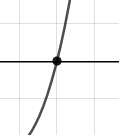
\includegraphics[width=0.3\textwidth]{../Figures/polyZeroBehaviorCopyDC.png}
    \end{center}\begin{enumerate}[label=\Alph*.]
\begin{multicols}{2}
\item 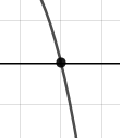
\includegraphics[width = 0.3\textwidth]{../Figures/polyZeroBehaviorCopyAC.png}
\item 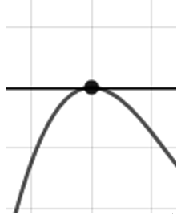
\includegraphics[width = 0.3\textwidth]{../Figures/polyZeroBehaviorCopyBC.png}
\item 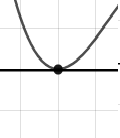
\includegraphics[width = 0.3\textwidth]{../Figures/polyZeroBehaviorCopyCC.png}
\item 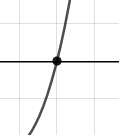
\includegraphics[width = 0.3\textwidth]{../Figures/polyZeroBehaviorCopyDC.png}
\end{multicols}\item None of the above.\end{enumerate}
\textbf{General Comment:} You will need to sketch the entire graph, then zoom in on the zero the question asks about.
}
\litem{
Describe the end behavior of the polynomial below.
\[ f(x) = -4(x + 6)^{4}(x - 6)^{5}(x + 2)^{5}(x - 2)^{5} \]The solution is the graph below, which is option A.
    \begin{center}
        \includegraphics[width=0.3\textwidth]{../Figures/polyEndBehaviorCopyAC.png}
    \end{center}\begin{enumerate}[label=\Alph*.]
\begin{multicols}{2}
\item \includegraphics[width = 0.3\textwidth]{../Figures/polyEndBehaviorCopyAC.png}
\item \includegraphics[width = 0.3\textwidth]{../Figures/polyEndBehaviorCopyBC.png}
\item \includegraphics[width = 0.3\textwidth]{../Figures/polyEndBehaviorCopyCC.png}
\item \includegraphics[width = 0.3\textwidth]{../Figures/polyEndBehaviorCopyDC.png}
\end{multicols}\item None of the above.\end{enumerate}
\textbf{General Comment:} Remember that end behavior is determined by the leading coefficient AND whether the \textbf{sum} of the multiplicities is positive or negative.
}
\litem{
Describe the end behavior of the polynomial below.
\[ f(x) = 4(x + 2)^{5}(x - 2)^{8}(x + 9)^{3}(x - 9)^{3} \]The solution is the graph below, which is option D.
    \begin{center}
        \includegraphics[width=0.3\textwidth]{../Figures/polyEndBehaviorDC.png}
    \end{center}\begin{enumerate}[label=\Alph*.]
\begin{multicols}{2}
\item \includegraphics[width = 0.3\textwidth]{../Figures/polyEndBehaviorAC.png}
\item \includegraphics[width = 0.3\textwidth]{../Figures/polyEndBehaviorBC.png}
\item \includegraphics[width = 0.3\textwidth]{../Figures/polyEndBehaviorCC.png}
\item \includegraphics[width = 0.3\textwidth]{../Figures/polyEndBehaviorDC.png}
\end{multicols}\item None of the above.\end{enumerate}
\textbf{General Comment:} Remember that end behavior is determined by the leading coefficient AND whether the \textbf{sum} of the multiplicities is positive or negative.
}
\litem{
Construct the lowest-degree polynomial given the zeros below. Then, choose the intervals that contain the coefficients of the polynomial in the form $x^3+bx^2+cx+d$.
\[ -5 + 5 i \text{ and } -1 \]The solution is \( x^{3} +11 x^{2} +60 x + 50 \), which is option B.\begin{enumerate}[label=\Alph*.]
\item \( b \in [-16, -10], c \in [59, 67], \text{ and } d \in [-58, -48] \)

$x^{3} -11 x^{2} +60 x -50$, which corresponds to multiplying out $(x-(-5 + 5 i))(x-(-5 - 5 i))(x -1)$.
\item \( b \in [4, 19], c \in [59, 67], \text{ and } d \in [46, 58] \)

* $x^{3} +11 x^{2} +60 x + 50$, which is the correct option.
\item \( b \in [-8, 6], c \in [-1, 13], \text{ and } d \in [3, 6] \)

$x^{3} + x^{2} +6 x + 5$, which corresponds to multiplying out $(x + 5)(x + 1)$.
\item \( b \in [-8, 6], c \in [-6, 3], \text{ and } d \in [-7, 3] \)

$x^{3} + x^{2} -4 x -5$, which corresponds to multiplying out $(x -5)(x + 1)$.
\item \( \text{None of the above.} \)

This corresponds to making an unanticipated error or not understanding how to use nonreal complex numbers to create the lowest-degree polynomial. If you chose this and are not sure what you did wrong, please contact the coordinator for help.
\end{enumerate}

\textbf{General Comment:} Remember that the conjugate of $a+bi$ is $a-bi$. Since these zeros always come in pairs, we need to multiply out $(x-(-5 + 5 i))(x-(-5 - 5 i))(x-(-1))$.
}
\litem{
Construct the lowest-degree polynomial given the zeros below. Then, choose the intervals that contain the coefficients of the polynomial in the form $ax^3+bx^2+cx+d$.
\[ \frac{-2}{5}, \frac{-3}{2}, \text{ and } \frac{1}{5} \]The solution is \( 50x^{3} +85 x^{2} +11 x -6 \), which is option C.\begin{enumerate}[label=\Alph*.]
\item \( a \in [48, 62], b \in [44, 50], c \in [-44, -38], \text{ and } d \in [1, 10] \)

$50x^{3} +45 x^{2} -41 x + 6$, which corresponds to multiplying out $(5x -2)(2x + 3)(5x -1)$.
\item \( a \in [48, 62], b \in [-106, -98], c \in [42, 50], \text{ and } d \in [-8, 2] \)

$50x^{3} -105 x^{2} +49 x -6$, which corresponds to multiplying out $(5x -2)(2x -3)(5x -1)$.
\item \( a \in [48, 62], b \in [79, 88], c \in [7, 18], \text{ and } d \in [-8, 2] \)

* $50x^{3} +85 x^{2} +11 x -6$, which is the correct option.
\item \( a \in [48, 62], b \in [79, 88], c \in [7, 18], \text{ and } d \in [1, 10] \)

$50x^{3} +85 x^{2} +11 x + 6$, which corresponds to multiplying everything correctly except the constant term.
\item \( a \in [48, 62], b \in [-85, -84], c \in [7, 18], \text{ and } d \in [1, 10] \)

$50x^{3} -85 x^{2} +11 x + 6$, which corresponds to multiplying out $(5x -2)(2x -3)(5x + 1)$.
\end{enumerate}

\textbf{General Comment:} To construct the lowest-degree polynomial, you want to multiply out $(5x + 2)(2x + 3)(5x -1)$
}
\litem{
Which of the following equations \textit{could} be of the graph presented below?

\begin{center}
    \includegraphics[width=0.5\textwidth]{../Figures/polyGraphToFunctionCopyC.png}
\end{center}


The solution is \( -13x^{8} (x + 3)^{10} (x + 2)^{5} \), which is option D.\begin{enumerate}[label=\Alph*.]
\item \( 14x^{10} (x + 3)^{10} (x + 2)^{5} \)

This corresponds to the leading coefficient being the opposite value than it should be.
\item \( 18x^{10} (x + 3)^{4} (x + 2)^{4} \)

The factor $(x + 2)$ should have an odd power and the leading coefficient should be the opposite sign.
\item \( -11x^{9} (x + 3)^{6} (x + 2)^{5} \)

The factor $x$ should have an even power.
\item \( -13x^{8} (x + 3)^{10} (x + 2)^{5} \)

* This is the correct option.
\item \( -8x^{11} (x + 3)^{10} (x + 2)^{10} \)

The factor $x$ should have an even power and the factor $(x + 2)$ should have an odd power.
\end{enumerate}

\textbf{General Comment:} General Comments: Draw the x-axis to determine which zeros are touching (and so have even multiplicity) or cross (and have odd multiplicity).
}
\litem{
Construct the lowest-degree polynomial given the zeros below. Then, choose the intervals that contain the coefficients of the polynomial in the form $x^3+bx^2+cx+d$.
\[ 4 - 3 i \text{ and } 3 \]The solution is \( x^{3} -11 x^{2} +49 x -75 \), which is option B.\begin{enumerate}[label=\Alph*.]
\item \( b \in [9, 12], c \in [40, 52], \text{ and } d \in [74, 86] \)

$x^{3} +11 x^{2} +49 x + 75$, which corresponds to multiplying out $(x-(4 - 3 i))(x-(4 + 3 i))(x + 3)$.
\item \( b \in [-14, -5], c \in [40, 52], \text{ and } d \in [-77, -72] \)

* $x^{3} -11 x^{2} +49 x -75$, which is the correct option.
\item \( b \in [0, 3], c \in [0, 5], \text{ and } d \in [-9, -8] \)

$x^{3} + x^{2} -9$, which corresponds to multiplying out $(x + 3)(x -3)$.
\item \( b \in [0, 3], c \in [-10, -6], \text{ and } d \in [7, 16] \)

$x^{3} + x^{2} -7 x + 12$, which corresponds to multiplying out $(x -4)(x -3)$.
\item \( \text{None of the above.} \)

This corresponds to making an unanticipated error or not understanding how to use nonreal complex numbers to create the lowest-degree polynomial. If you chose this and are not sure what you did wrong, please contact the coordinator for help.
\end{enumerate}

\textbf{General Comment:} Remember that the conjugate of $a+bi$ is $a-bi$. Since these zeros always come in pairs, we need to multiply out $(x-(4 - 3 i))(x-(4 + 3 i))(x-(3))$.
}
\litem{
Describe the zero behavior of the zero $x = 3$ of the polynomial below.
\[ f(x) = 3(x - 3)^{5}(x + 3)^{10}(x + 8)^{5}(x - 8)^{6} \]The solution is the graph below, which is option D.
    \begin{center}
        \includegraphics[width=0.3\textwidth]{../Figures/polyZeroBehaviorDC.png}
    \end{center}\begin{enumerate}[label=\Alph*.]
\begin{multicols}{2}
\item \includegraphics[width = 0.3\textwidth]{../Figures/polyZeroBehaviorAC.png}
\item \includegraphics[width = 0.3\textwidth]{../Figures/polyZeroBehaviorBC.png}
\item \includegraphics[width = 0.3\textwidth]{../Figures/polyZeroBehaviorCC.png}
\item \includegraphics[width = 0.3\textwidth]{../Figures/polyZeroBehaviorDC.png}
\end{multicols}\item None of the above.\end{enumerate}
\textbf{General Comment:} You will need to sketch the entire graph, then zoom in on the zero the question asks about.
}
\end{enumerate}

\end{document}